%\chapter{Etude des besoins et contraintes dans les visites touristiques}
\chapter{Les enjeux de l'interaction dans les visites touristiques}
\label{chap:etude}

INTRO chapitre : les nouveaux moyens d'interaction et d'accès à l'information, dans le cadre des musées et sites touristiques, donc avec les contraintes qui vont avec. Egalement les contraintes liées à GUIMUTEIC; comme le coup, la générailisation et la facilité d'installation. On va donc regarder quel type d'actions sont voulu par les utilisateurs, quels gestes leurs semble nécessaires et utile.


L'objectif de ce travail de thèse est de fournir une réponse aux problématiques d'accès à l'information pendant les visites touristiques. 
Pour cela, nous allons étudier les possibilité de mise en place d'un système d'interaction avec l'utilisateur au sein des musées.
Lorsque l'on parle de dispositifs pour l'aide à la visite dans les musées et sites touristiques, deux types de besoins et contraintes sont en prendre en compte, au niveau du musée et au niveau de l'utilisateur.


\section{Les nouveaux moyens d'interaction et d'accès à l'information}

Les musées veulent de nouveaux moyens d'interaction. (trouver références)
Les utilisateurs aussi (autre ref)
Exemple de musées avec des interaction physique, ou de position.


Museum Informatics
Paul F. Marty
College of Communication and Information, Florida State University, Tallahassee, Florida, U.S.A.
Abstract
Museum informatics is the study of the sociotechnical interactions that take place at the intersection of
people, information, and technology in museums. This entry presents an overview of museum informatics,
covering such topics as information representation, information organization and access, information
management, information technology, information interactions, and information professionals in
museums. It explores the impact of information science and technology on museums, museum professionals,
and museum visitors, and argues that museum researchers must take a sociotechnical approach to
studying the use of information resources and technologies in museums.
http://marty.cci.fsu.edu/preprints/marty_elis2010.pdf

Effective Levels of Adaptation to Different Types
of Users in Interactive Museum Systems
F. Paterno` and C. Mancini
CNUCE-C.N.R., Via S. Maria 36, 56126 Pisa, Italy. E-mail: fpaterno@cnuce.cnr.it
Users interact with museum application interfaces for
many reasons. There are various types of users, who
want to perform various tasks, in various contexts, that
can access the same Web site. Thus, it is important to
have user interfaces able to adapt to these different user
requirements to facilitate the accomplishment of the
desired goals. Most current interfaces to museum information
do not take into account this variety of types of
users, thus providing interfaces that some users find
confusing to achieve their goals. In this article we discuss
the various possible levels of support that can be
given to different users during navigation of museum
information. In particular, we focus our attention on how
to obtain adaptable and adaptive interfaces using the
web site for the Marble Museum, which we have designed
and developed, as a source
http://starlings.co.kr/ucc/classroom/1438320120529172910.pdf



The iPhone and Its Use in Museums
As with other cultural institutions, museums have always
been ascribed specific roles in society. Throughout the years,
these roles have not changed dramatically, even though the
means to fulfill them have. As Tony Bennett convincingly
documented in his book The Birth of the Museum, the museum
was from its very beginning meant to enlighten and educate
the public, while serving as the temple of the arts in an elitist
fashion. Furthermore, the museum served as an instrument
of the disciplinary society, where people from different social
classes met. Ideally, the lower classes could learn from the
“correct” behavior of the upper classes. Finally, in a similar
Foucaultian fashion, the museum could filter out certain
knowledge, thereby prioritizing certain historical readings,
artifacts, and knowledge instead of other alternative options
(Bennett 1995).
https://www.researchgate.net/profile/Rich_Ling/publication/259257980_The_iPhone_and_its_use_in_museums/links/560883a808ae5e8e3f3a8bbd/The-iPhone-and-its-use-in-museums.pdf


\begin{figure}%
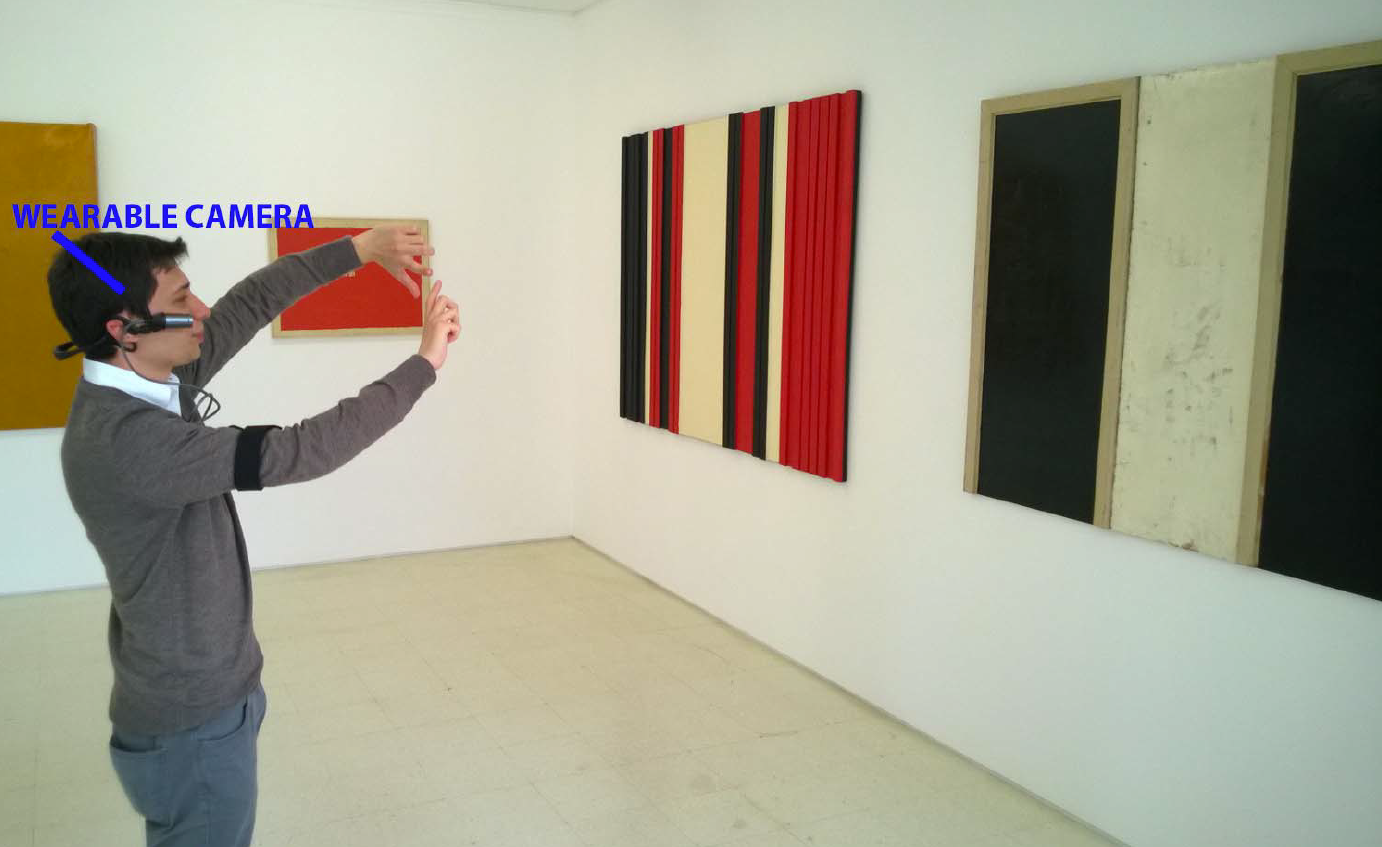
\includegraphics[width=\columnwidth]{figures/wearable.PNG}%
\caption{Exemple d'une interaction à base de geste en face d'une oeuvre. (Source)}%
\label{exempleGesteMusee}%
\end{figure}


\section{Les contraintes des musées et du projet GUIMUTEIC}

Tout ça est limité par les musées eux-mêmes. Les oeuvres d'art doivent être le truc principale, on ne peut pas se permettre d'avoir d'autre chose afficher visible par l'utilisateur (exemple de l'extincteur?)



\section{Une interaction à base de geste}

Pour déterminer les interactions intéressante pour notre projet, nous avons réaliser un certains nombre de séance de conception participative.
Celles-ci permettent, grâce à des exercices ludiques, de définir les usages futurs d’un dispositif innovant auprès des utilisateurs finaux. 

La figure~\ref{fig:photoGestes} montre les cinq gestes statiques définis par les séances de conception.

\begin{figure}%
	\label{fig:photoGestes}%
	\begin{minipage}[c]{.32\linewidth}
		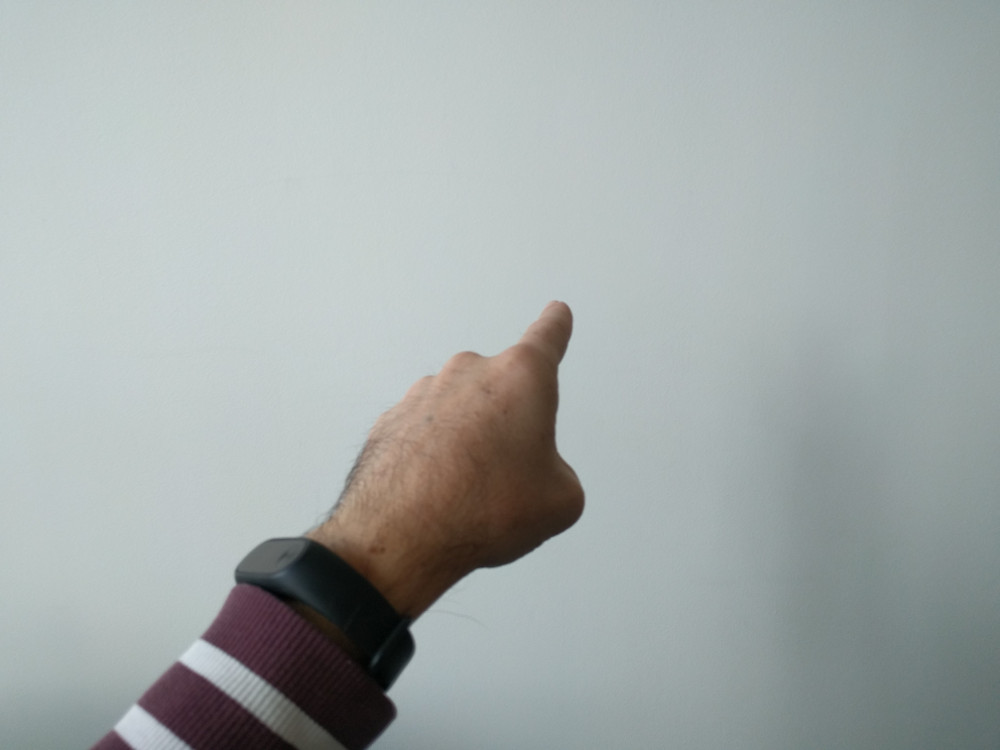
\includegraphics[width=\columnwidth]{figures/1.jpg}%
		\caption*{Pointer}%
	\end{minipage} \hfill
	\begin{minipage}[c]{.32\linewidth}
		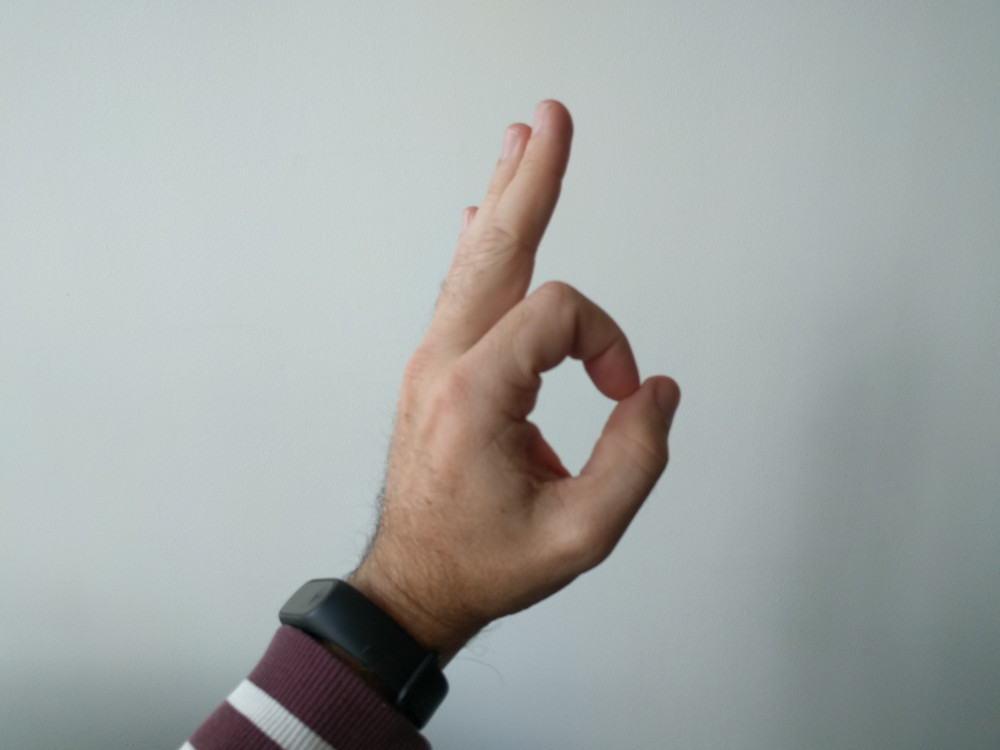
\includegraphics[width=\columnwidth]{figures/2.jpg}%
		\caption*{OK}%
	\end{minipage} \hfill
	\begin{minipage}[c]{.32\linewidth}
		
\includegraphics[width=\columnwidth]{figures/3.jpg}%
		\caption*{Valider}%
	\end{minipage}
	\centering
	\begin{minipage}[c]{.32\linewidth}
		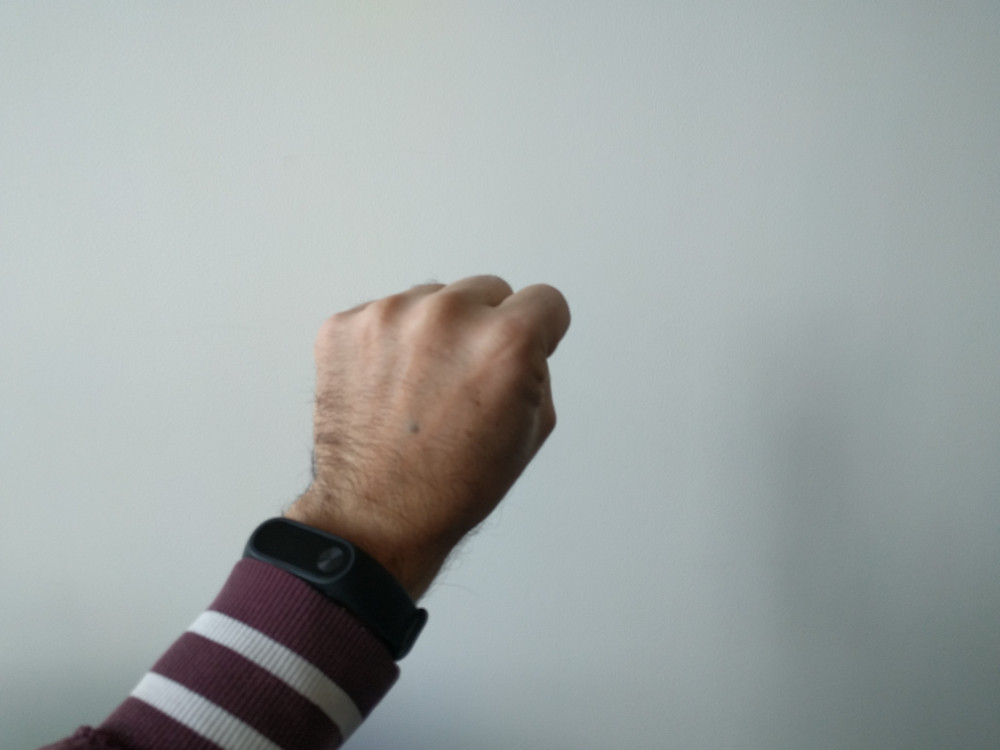
\includegraphics[width=\columnwidth]{figures/4.jpg}%
		\caption*{arrêter}%
	\end{minipage}
	\begin{minipage}[c]{.32\linewidth}
		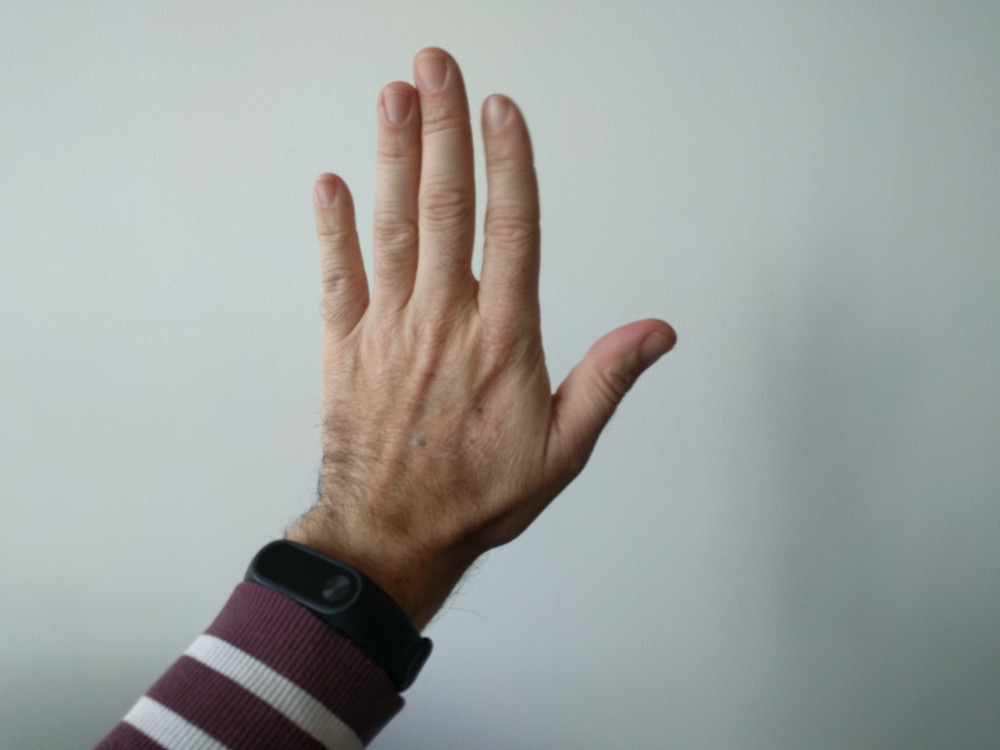
\includegraphics[width=\columnwidth]{figures/5.jpg}%
		\caption*{stop}%
	\end{minipage}
	\caption{Exemple des gestes mis en avant par les séances de conceptions participative.}
	
\end{figure}

Un corpus de vidéos de gestes a été réaliser dans le but d'évaluer les systèmes developpés dans ce projet. Ce cropus est composé de vidéo en vue à la première personne, prise dans différentes conditions, et également devant un fond vert, ppour permettre de générer de nouvelles données. La description complète du corpus est disponible dans l'annexe~\ref{chap:corpus}.

\section{Le système GUIMUTEIC}


\begin{figure}%
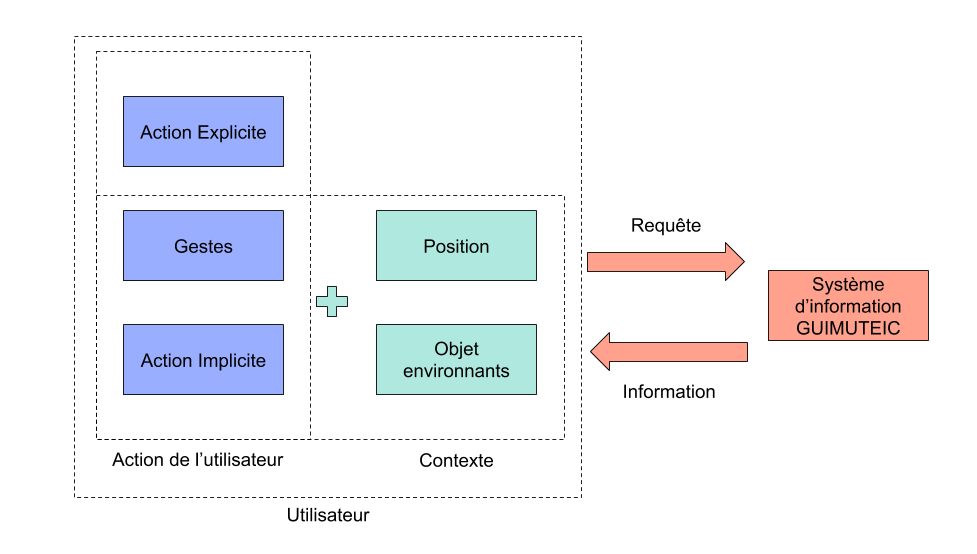
\includegraphics[width=\columnwidth]{figures/ActionContexte.png}%
\caption{Schémas d'organisation du sytème d'information GUIMUTEIC. Les différentes actions possibles de l'utilisateur dans la colonne de droite peuvent être couplées au information sur le contexte pour emettre une requête au système d'information, et avoir ou non une information.}%
\label{fig:actioncontexte}%
\end{figure}






	
	
	%Il est possible notamment d'avoir pour chaque musée un certains nombre d'image, du photo, de chaque oeuvre. Il n'est par contre pas envisageable pour chacun des musée de faire des vidéos de visite complètes, annotée, avec les oeuvres identifiée à chaque instance.
%Tout système produit dans le projet, doit donc tenir compte de cette limitation.
%Plus la base de données requise doit être précise, plus la mise en place du système sera compliqué. Les prises de vue et leur annotations doit donc être aussi limité que possible.
%
%Certain éléments ne peuvent donc pas être présent dans la base de données. Dans le cas d'un corpus d'image, il n'est pas envisageable d'avoir une annotation des régions de l'image où se situe l'objet, mais seulement une annotation au niveau de l'image entière. 
%De même, créer une base de données de vidéo est dans ce cas précis, un problème. Nous avons tout de même décider de nous baser sur un ensemble de vidéos annotées par séquence, avec seulement une information indiquant quel objet est présent dans cette séquence. Cela représente le niveau minimal d'annotation sur les vidéos.
%
%
%
%Afin de faciliter la lecture, nous appelons abusivement dans la suite ``{\it œuvre}'' tout objet présenté dans un musée, tout en sachant que l'on dépasse le cadre strict des artefacts (i.e. objets fabriqués par l'Homme), comme les musées dédiés aux roches par exemple.


